\setcounter{chapter}{1} %this gives Chapter 2
\chapter{Numerical
 modelling of multiple-electrode traps}
\label{chapter:simulation}

To predict the behaviour of ion traps, generally computer models of the traps are created and their operation is simulated. This chapter discusses this modelling, the particular ion trap designs used in our research group and results of simulations of two previously untested designs. 
Further information on the software is continued in the appendices.


\section{Ion trap modeling}

The main aim of a numerical  model of an ion trap is the prediction of potentials created by DC and radio-frequency voltages applied to the electrodes. The highest frequency RF fields used are of order $10\MHz$, thus wavelengths are of order $10\m$. Since the characteristic size of the ion traps is $<1\mm$, quasi-static modelling is a good approximation. 

There are two widely used methods to solve Laplace's equation in the region around an ion trap: the Finite Element Method (FEM) and the Boundary Element Method (BEM). Both find approximate solutions of partial differential equations. In FEM, the whole volume of interest (the electrodes and the free space in between them) is subdivided into a discrete mesh of nodes. The nodes are connected to their neighbours by linear or quadratic functions. An energy minimization algorithm is then used to calculate the potential on the mesh, subject to boundary conditions (voltages applied to the electrodes). 

The BEM attempts to solve partial differential equations by  forming them into integral equations. As opposed to FEM, in BEM only the surfaces are subdivided. The method uses boundary conditions to find the boundary values to the integral equations. When the BEM is applied to ion traps, one finds the charge distribution on the electrodes subject to electrode geometry and applied voltages. Then the potentials can be calculated at arbitrary positions in the space between the electrodes. 

Each method has advantages and disadvantages. Since in BEM only surfaces are discretized as opposed to volume discretization in FEM, BEM scales better when larger structures are modelled. However, because in FEM only neighbouring nodes are connected, the matrix describing the system of equations of the model is very sparse; the number of non-zero elements in the matrix scales as $O(n)$ with the number of nodes $n$. In BEM all subdivisions of an object (such as an electrode) are described by joint boundary conditions. Thus, the matrix describing the model is usually densely-packed, and the number of non-zero elements in the matrix scales as $O(n^2)$. 
In BEM, the potential can be calculated at arbitrary positions, while in FEM the potential is given only at the nodes and approximated in between. FEM can incorporate material inhomogeneities, while the BEM only deals with linear homogeneous materials. 

Due to these differences, the efficiency and speed of the calculations is highly dependent on the design to be modelled. Both methods have several implementations (FEM: Opera\footnote{Vector Fields Opera, \url{http://www.vectorfields.com/}},SIMION\footnote{Scientific Instrument Services, Inc., \url{http://www.simion.com/}}; BEM: CPO\footnote{Charged Particle Optics, SIS Inc., \url{http://www.simion.com/cpo/}}). For ion traps with relatively simple geometry and small/medium number of electrodes, the BEM method proved to be efficient, and the results presented here were obtained using Charged Particle Optics (CPO) by Scientific Instrument Services. 

Due to the linear nature of Laplace's equation, potentials generated by the different electrodes are independent and can be calculated separately. Generally, unit voltage is set on a selected electrode $i$, while all other electrodes are grounded. The potential $\phi_i(\vec{r})$ is then calculated at the position of interest $\vec{r}$. The calculation is repeated with all other electrodes. This procedure is the same for both DC and RF electrodes, because of the quasi-static approximation. The electric potential set up by a given voltage configuration is then given by
\be
\phi(\vec{r},t) = V_{\rm rf}\phi_{\rm rf}(\vec{r})\sin(\Omega_{\rm rf} t) + \sum_i V_i \phi_i (\vec{r})
\label{eq:fulltrappot}
\ee
where $V_{\rm rf}$ and $V_i$ are the voltages on the RF electrode and DC electrodes, and $\Omega_{\rm rf}$ is the RF drive frequency. Equation~\ref{eq:fulltrappot} is used when a complete description of the ion's motion (both secular and micromotion) is sought. If only the secular motion of the ion is of interest, the effect of the RF field on the secular motion can be approximated by the RF pseudopotential
\be
U_p(\vec{r}) = \frac{q^2 V_{\rm rf}^2}{4m\Omega_{\rm rf}^2}|\nabla \phi_{\rm rf}(\vec{r})|^2
\label{eq:pseudopot}
\ee
where $q$ and $m$ are the charge and  mass of the ion. Thus the complete expression for the potential energy in the pseudo-potential approximation is
\be
\Phi_p(\vec{r},t) = \frac{q^2 V_{\rm rf}^2}{4m\Omega_{\rm rf}^2}|\nabla \phi_{\rm rf}(\vec{r})|^2 + q \sum_i V_i \phi_i (\vec{r})
\label{eq:pseudopotcomplete}
\ee

The simulations were performed as follows. A model of the trap was created in the structural description language of CPO.  Locations of interest were chosen, e.g., positions along the trap axis, or points to represent 2D cross sections in the radial direction at different positions along the trap axis. We then proceeded as above; setting the voltage of a single electrode to unity while keeping everything else grounded we calculated $\phi_i(\vec{r})$ for one electrode at the locations of interest. This process was repeated for all electrodes (both DC and RF). The resulting potential was stored in a database, and was used in a numerical computation software, such as Matlab\footnote{The MathWorks, Inc., \url{http://www.mathworks.com/}} or GNU Octave\footnote{GNU Octave, \url{http://www.gnu.org/software/octave/}} to calculate the potentials at the location of interest for arbitrary voltage configuration on the electrodes, as needed by the experiments.


\section{Trap designs}

The evolution in ion trap design can be illustrated by the different ion traps that are in use and are planned in our research group. 

Macroscopic traps are manually assembled, and have ion-electrode separation of order $\approx 1\mm$. Advantages of macroscopic traps include generally a low heating rate and a large trap depth which result in very long ion lifetimes. The design is tried and tested, and the trap is relatively cheap to produce. Its disadvantages are its lack of scalability to a large number of ions due to its single trapping region and the difficulty of achieving high trap frequencies because of the large voltages required as a consequence of the large electrode-ion distances. The first ion trap in our research group, a linear Paul trap, is an example of a macroscopic trap (see \cite{Barton2000}).

Mesoscopic traps present a transition stage between traditional style traps with a single trapping region and microscopic traps with good scalability. Built using traditional methods, they nevertheless can have multiple trapping regions and provide a testing ground of procedures being developed for microscopic traps. However, the manual assembly can be a  weak point because imprecisions have a magnified effect as the ion trap design is scaled down in size. The Liverpool trap, described in the next section, is a mesoscopic ion trap.

The smallest kind are microscopic ion traps. They can have very high trap frequencies even with low electrode voltages, a large number of trapping regions for dealing with multiple ions, and precise manufacturing by microfabrication methods. However, while some of the microfabrication methods are well-established (e.g. because of their use in computer chip manufacturing industry), some are highly experimental and can have a significant error-rate. Another disadvantage is the smaller trap depth and higher heating rate compared to larger traps. Small scale production of microscopic traps is very expensive, but a successful mass-produced design would be much cheaper. Examples of microscopic traps include the Sandia trap (see Section~\ref{sec:sandiaintro}), and the traps designed by the MICROTRAP Consortium\footnote{MICROTRAP Consortium, \url{http://www.microtrap.eu/}}.

\section{The Liverpool trap}

The Liverpool trap (see Figure~\ref{fig:liverpooltrap}) was built by S. Taylor and B. Brkic from the University of Liverpool. Its electrodes are machined from non-magnetic stainless steel, and separated by Macor (a type of machinable glass ceramic) spacers. It is a three layer-design, with DC electrode ``fingers'' in the middle layer and RF electrodes below and above. A set of 4 compensation electrodes is also present to adjust for stray fields, mostly in the direction perpendicular to the plane of the DC electrodes (Y direction). 

\begin{figure}[!t]
\begin{center}
$\begin{array}{cc}
\mbox{\bf (a)} & 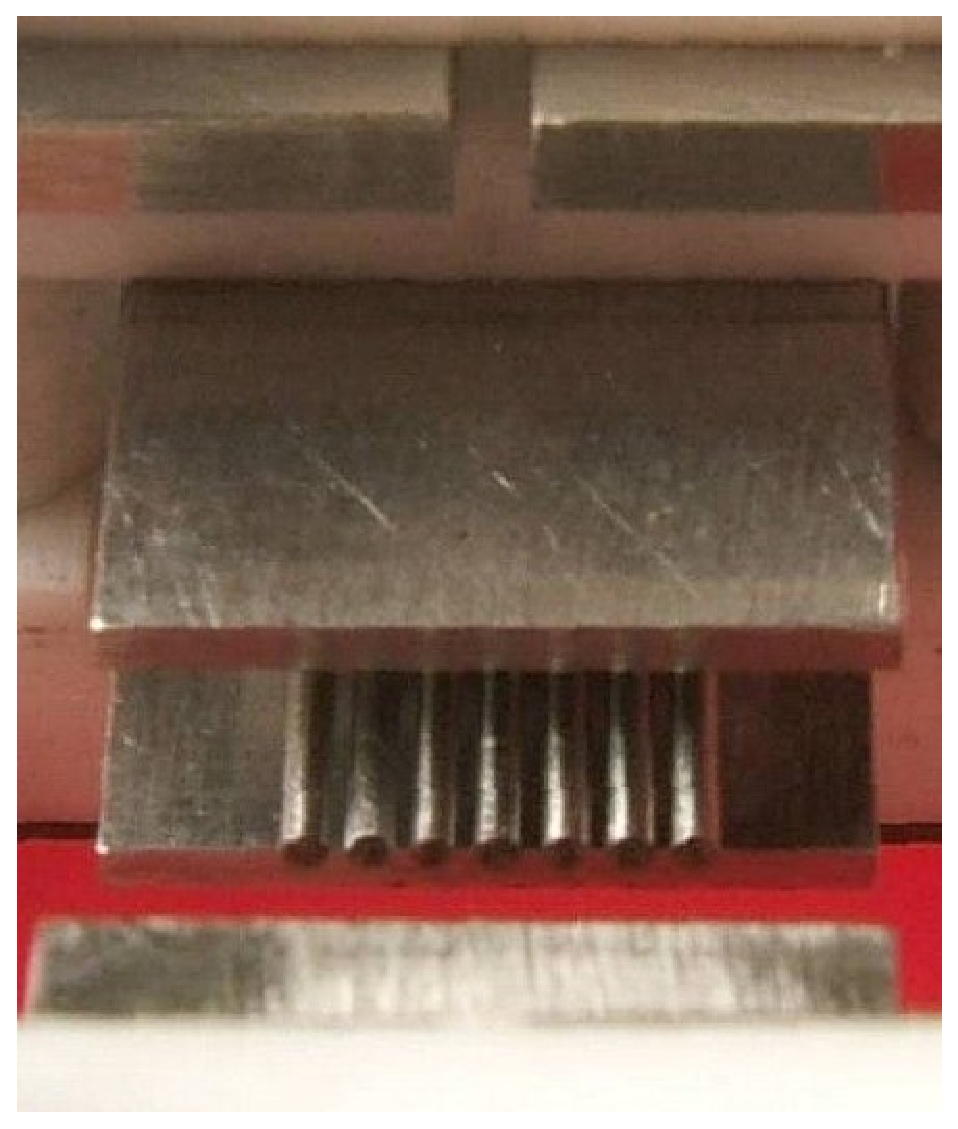
\includegraphics[width=6cm]{chapter2/liverpool/liverpool3}\\
\mbox{\bf (b)} & 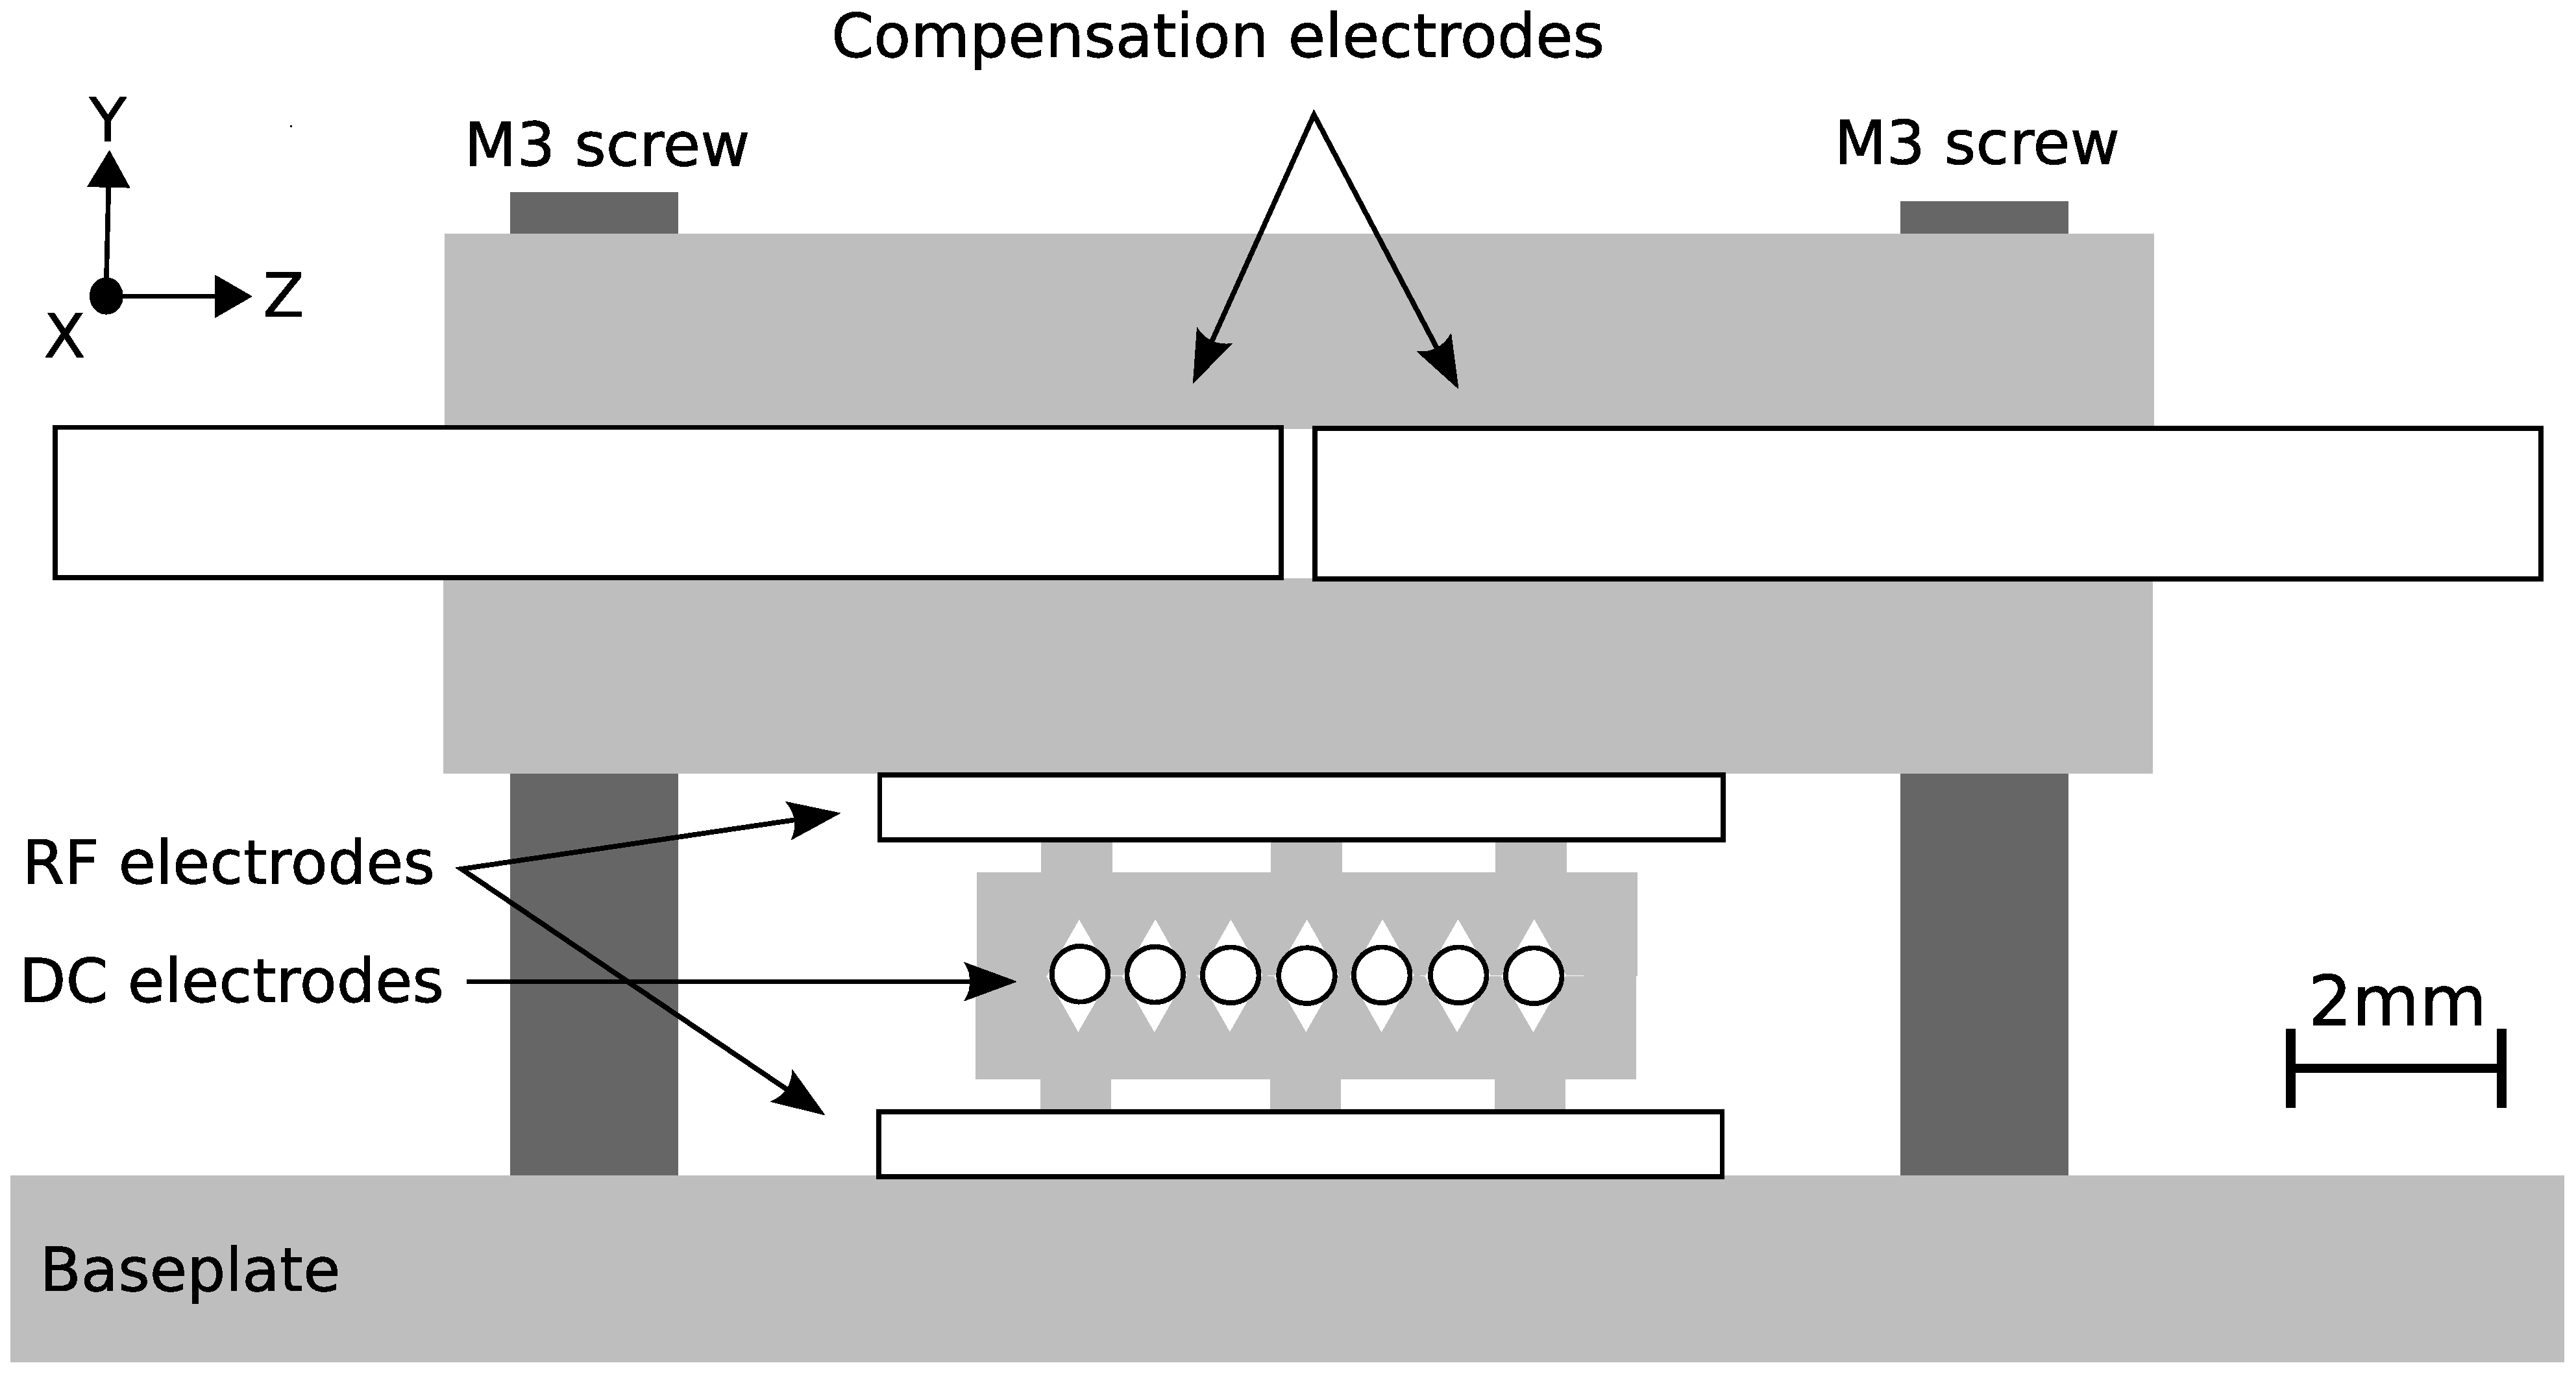
\includegraphics[width=11cm]{chapter2/liverpool/liverpoolsheme_v3} \\
\end{array}$
\end{center}
\caption[Liverpool trap photo and schematics]{a) A view of the Liverpool trap, b) Cross-section of the trap. The DC electrodes are specified to have a nominal diameter of 0.5775\mm, and axis-to-axis separation of 0.7525\mm. The electrodes are separated by machined Macor blocks (light gray areas on the plot), and the structure is assembled using M3 non-magnetic steel screws (dark gray). The smallest ion-electrode distance is 0.7\mm.}
\label{fig:liverpooltrap}
\end{figure} 


\subsection{Design of the trap}

The Liverpool trap has an unusual design. Most experiments involving the transport of ions among multiple trapping zones have adopted a design philosophy in which the RF potential is as smooth as possible. To achieve this one can, for example, make the DC electrodes have the shape of a single long electrode, extending either side of the trap axis Z, interupted by narrow cuts to make the segments. This allows structure to be introduced in the DC potential as a function of Z, while the RF ground at these electrodes is consistent with a smooth RF potential, almost without variation in the Z direction. 

A problem that arises with small traps, however, is electric field breakdown. One wants to have tight trapping potentials, but if the DC electrodes are close to one another and have sharp edges then the problems of field emission and breakdown of insulating surfaces are exacerbated. This issue was studied theoretically in \cite{Home2006a}, and a number of trap geometries were modelled. The issue of trap tightness arises especially when one wants to split apart or join together strings of ions. During such a ``split'' or ``splice'' operation, 
the potential as a function of $z$ must change from the usual simple quadratic function to a quartic function, so that two wells with a barrier in between them can be formed. To achieve this without reducing the confinement places 
the most stringent conditions on the electric field breakdown. Therefore in \cite{Home2006a} a geometric factor $\gamma$ was defined as
\begin{equation}
\gamma = \frac{\beta \rho^3}{E_{\rm max}}
\label{eq:gammadef}
\end{equation}
where $\beta$ is the coefficient of the quartic term in the DC potential $\sum_i V_i \phi_i(z)$ along the trap axis at the origin, $\rho$ is the distance of the origin to the nearest electrode surface, and $E_{\rm max}$ is the largest electric field at any electrode surface. By this measure, a ``good'' trap structure would have a high value of $\gamma$.

Another important issue is the tightness of the RF confinement. In large traps this is typically limited by the size of the available RF voltages, but  in a small trap the voltages are manageable and again electric field breakdown 
presents an important limit. This can be characterised by another geometric factor 
\begin{equation}
\mu = \frac{Q_{\rm ac} \rho}{E_{\rm max}}
\label{eq:mudef}
\end{equation}
where $Q_{\rm ac}$ is the coefficient of the quadratic term in the potential $\phi_{\rm rf}$ generated by the RF electrodes at the trap centre.

In \cite{Home2006a} it was shown that a geometry that achieves a good combination of values for these geometric factors consists of a row of DC ``fingers'' nearest to the trap axis, with RF electrodes above and below and set back somewhat. It is this geometry that the Liverpool trap was designed to realise. This trap is not microfabricated. It has a larger (of order 1 mm) scale, so will not suffer from electric field breakdown at the voltages we can achieve, but it will enable us to test whether this approach is viable. In particular, this type of geometry results in much more structure in the RF potential along Z than is the case in the ``traditional'' approach. This means the ions will undergo considerable micromotion at most positions along the trap axis. We will be able to test whether 
this micromotion in practice leads to problems when ions are moved along the trap axis, or when ion strings are split and recombined. 

In the pseudopotential model, the RF oscillation is perfectly harmless: it merely contributes to the total potential experienced by the ion and thus influences the location of the ``trap centre'' at any given configuration of the DC voltages. Numerical modelling taking the RF oscillation into account also suggests that it need not be a problem. However, practical experience with trapped ions has given evidence, albeit inconclusive, that micromotion can be associated with heating or other problems. It is not yet known whether or not this will prove to be a significant issue, so it is one aim of the planned work with the Liverpool trap to resolve this. 

In the next section we will present the main characteristics of the trap, such as the expected potential in the radial and axial directions, as a function of position along the axis, and comment on how the DC voltages are chosen to realise a given desired situation. We also briefly study the issue of manufacturing imprecision.

\subsection{Analysis of trap geometry}
\label{sec:liverpoolgeom}
Figure~\ref{fig:trapmodels} shows the trap's computational model, looked at from the Y direction. The first version (Figure~\ref{fig:trapmodels}, left) corresponds to the originally intended design, and used for benchmark calculations, to explore the expected behaviour of the Liverpool trap.

As an illustration, Figure~\ref{fig:liverpoolfields} shows the calculated electric field potential in the $X-Y$ plane at the trap centre, when the DC electrodes are grounded and the RF electrodes are at the set voltage. 

Figure~\ref{fig:liverpoolvolts} shows a calculation of voltages on the DC electrodes to produce a single $\omega_{\rm dc}/2\pi = 1\MHz$ potential well at an arbitrary position along the trapping axis (the Z direction). The RF voltages are not included because in the ideal situation the RF field has no component in the axial direction. The computational model can be used to derive the voltage configuration in the case of different constraints, such as 2 or 3 trapping regions (instead of only 1) or with different oscillation frequencies. This is useful in the ion-shuttling experiments, for example.



\begin{figure}[!t]
\begin{center}
$\begin{array}{cc}
\includegraphics[width=7.5cm]{chapter2/liverpool/trapmodel_ideal_v2} & 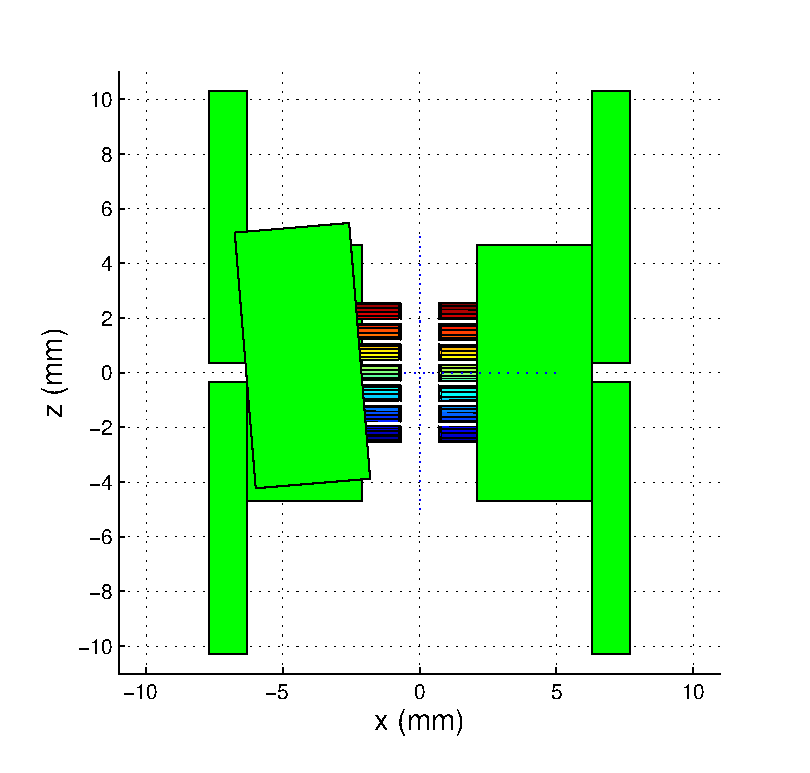
\includegraphics[width=7.5cm]{chapter2/liverpool/trapmodel_twist_v2} \\
\end{array}$
\end{center}
\caption[Computer model of Liverpool trap, with twisted RF electrode]{Computer models of the Liverpool trap, as  used in the simulations. The trap is viewed from above (along the Y axis, see Figure~\ref{fig:liverpooltrap} for note on directions). (Left) The Liverpool trap as it was designed. (Right) The trap with one of the RF electrodes twisted and displaced, as it was found to be after assembly. The electrode is displaced by $\Delta z \approx 0.9\mm$,$\Delta y \approx 0.3\mm$ and twisted by $\theta \approx 4.7\degree$ in the X-Z plane. The model is based on photographs taken of the trap. \cversion}
\label{fig:trapmodels}
\end{figure} 

\begin{figure}[!t]
\centering
%\includegraphics[width=9cm]{chapter2/liverpool_contours_v1_2}
%\includegraphics[width=9cm]{chapter2/liverpool_contours_v1_3}
\includegraphics[width=9cm]{chapter2/liverpool_contours_v1_4}
\caption[Calculation of electric field in the Liverpool trap]{Electric field due to a fixed voltage on the RF electrodes in the Liverpool trap. Cross section in the X-Y plane, as shown in Figure~\ref{fig:liverpooltrap}b.}
\label{fig:liverpoolfields}
\end{figure} 


\begin{figure}[!t]
\centering
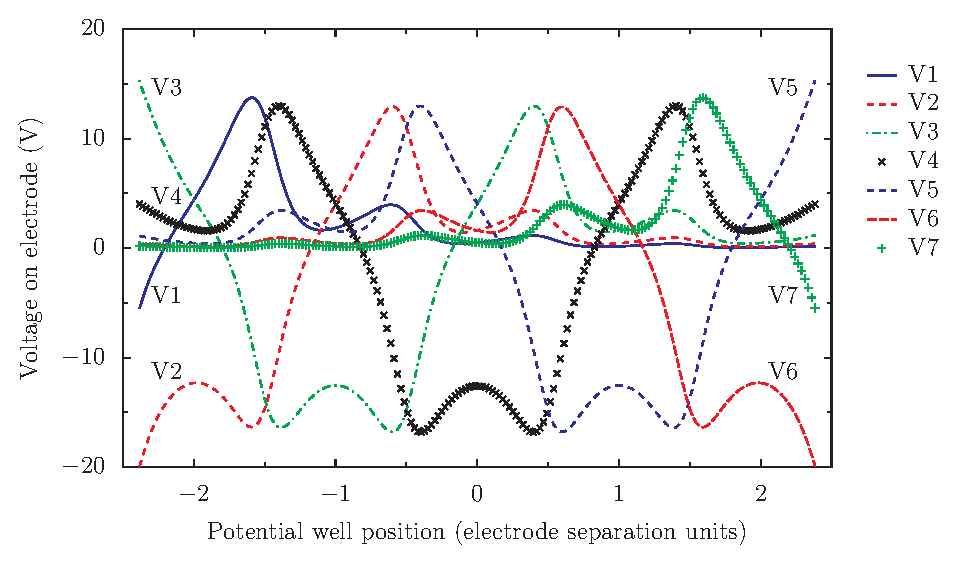
\includegraphics[width=14cm]{chapter2/liverpool/vcalc_allelectrodes}
\caption[Voltages on DC electrodes of Liverpool trap]{Voltages on electrodes to generate a single DC potential well with $\omega/2\pi = 1\MHz$ as a function of well position along the axis. Position is shown relative to the centre positions of the 7 DC electrodes. The electrode-electrode separation is nominally 0.7525\mm. Positions left of electrode -2 and right of electrode +2 are not shown, as it is not possible to trap in those regions. \cversion}
\label{fig:liverpoolvolts}
\end{figure} 


The geometric factors $\gamma$ and $\mu$, defined in Equations \ref{eq:gammadef} and \ref{eq:mudef} respectively, can  also be calculated. One finds
\begin{align}
\gamma & \simeq 0.02,\\
\mu & \simeq 0.146.
\end{align}
The Liverpool trap was designed to have high $\gamma$ value compared to other traps (see e.g. Section~\ref{sec:sandiaintro}), which facilitates ion pair splitting. 

%%%%%%%%%%%%%%%%

A point of interest is the effect of the segmented DC electrodes on the RF field along the trapping (Z) axis. The main effects can be understood by expanding the RF potential at any point $z_0$ as a power series in $z-z_0$, and examining the first few terms:
\be
\phi_{\rm rf}(z) \simeq \phi_{\rm rf}(z_0) + a (z-z_0) + b (z-z_0)^2
\ee
where
\be
a = \left. \frac{ \der \phi_{\rm rf} }{\der z} \right|_{z_0}, \;\;\;\;
b = \frac{1}{2} \left. \frac{ \der ^2 \phi_{\rm rf} }{\der z^2} \right|_{z_0}.
\label{eq:rfcoeffs}
\ee
The size of the oscillating electric field is given by $a$. It is important because it causes micromotion, see Figure~\ref{fig:rfaxialeffect} (right). The micromotion maximum velocity reaches some hundreds of \mps\, at the extreme trapping positions, under typical operating conditions. This will complicate laser interactions with the ions at those locations, suggesting that they could be used for storing ions temporarily but not for logical quantum gate operations.

In the pseudo-potential approximation (Equation~\ref{eq:pseudopot}), the contribution to the potential energy (i.e. the function describing the secular motion) is proportional to 
\be
\left| \nabla \phi_{\rm rf} \right|^2 = a^2 + 2 a b (z-z_0) + 4 b^2(z-z_0)^2
\ee
The constant offset $a^2$ has no effect on the motion. The linear term represents a force which displaces the local trapping centre slightly away from the location calculated from the d.c. potential alone; the quadratic term represents a (small) increase in the confinement along Z.

Figure~\ref{fig:rfaxialquad} shows the quadratic coefficient as a function of $z$. At electrode positions 2 and -2 the effect is to increase the secular frequency from 300\kHz\, (DC well) to 320\kHz\, (DC plus RF). Figure~\ref{fig:rfaxialeffect} (left) shows the displacement of the trapping centre away from that calculated from the DC potential, when the vibrational frequency in the DC potential well is 300\kHz. It is seen that the displacement is a small correction that needs to be taken into account.



%%%%%%%%%%%%%%%%




%A point of interest is the effect of the segmented DC electrodes on the RF field along the trapping $Z$ axis. Figure~\ref{fig:rfaxialeffect}(left) shows the calculated axial quadratic coefficient by the RF electrodes. Several bumps are visible at the positions of the DC electrodes. Due to this non-flat axial RF field the ion's motion will be different from the ideal situation. The pseudo-potential centre is at $Z=0$, thus when the ion is trapped at a position different from the centre, it will have micromotion due to imperfect compensation. To estimate the effect of such imperfect compensation, the micromotion maximum velocity was calculated for different trapping positions along the $Z$ axis (see Figure~\ref{fig:rfaxialeffect}). The DC trapping frequency was set to $\omega_{dc}/2\pi = 300 \kHz$, the maximum voltage on the RF electrode  to $V_{rf} = 200V$ and the RF drive frequency to $\Omega/2\pi = 5.92\MHz$, which are typical operating parameters. The results show, that the micromotion, reaching more than 450\mps\, furthest from the centre, presents a difficulty e.g for ion shuttling or ion pair splitting operation off-centre.


%%%%One point of interest about the trap's behaviour is the effect of no direct line of sight between the RF-electrode and the trapped ion. Because of the requirements of wide optical access, the RF electrodes are displaced away from the trapping region compared to the DC electrodes. In effect the RF electrodes are shielded from the trapped ion by the DC electrodes.  Figure~\ref{fig:rfaxialeffect}(left) shows the quadratic coefficient of the basis function of the pseudo-potential ($|\bigtriangledown \phi_{rf}(z)|^2$, see equation~\ref{eq:pseudopot}) as a function of the location along the trap axis ($Z$). Ideally, the RF electrodes should have zero potential gradient in the $Z$ direction, but this would only be true in case of infinite electrodes. In Figure~\ref{fig:rfaxialeffect}(left) the effect of the shielding is visible as bumps in the function at the locations of the DC electrodes. This shielding can cause problems in the outer regions of the trap, close to electrodes $\pm 3$ (\#1 and \#7). The shielding becomes highly asymmetric: consider an ion trapped in front of electrode \#2 (or -2 in the notation of the plot). In one direction there are 5 other electrodes shielding from the RF field, while in the other direction there is only a single DC electrode, and the RF electrode is close to having a line of sight to the ion. Because of this asymmetry, the gradient of the potential generated by the RF electrode increases, and starts to influence the ion's axial motion.
%
%It is possible to estimate the effect of this asymmetry. Given a potential well at a particular position along the $Z$ axis, the pseudo-potential model can be used to calculate how much the ion is displaced by the RF field. Figure~\ref{fig:rfaxialeffect}(right) shows the location of the pseudo-potential minimum along the $Z$ axis, as a function of the position of the DC potential well. The effect is calculated for $V_{rf} = 200V$ and $\Omega/2\pi = 5.92\MHz$, which correspond to standard experimental settings. The radial frequencies are then $\omega_{RF}/2\pi \approx 1\MHz$. The potential well due to the DC voltages alone had $\omega_{DC}/2\pi = 300\kHz$ axial frequency. Under these conditions, significant influence from the RF field in the $Z$ direction is predicted near electrodes $\pm 2$, while the region in between electrodes $\pm 1$ is not significantly affected.

%In principle, stronger DC confinement compared to the RF field (higher $r = \omega_{DC} / \omega_{RF}$ ratios) would improve the situation. However it might not be possible to increase the ratio significantly. For reliable trapping  $r < 0.5$ is desirable \textit{(ref)}. In the case of the calculation presented in Figure~\ref{fig:rfaxialeffect}, $\omega_{RF}/2\pi \approx 1\MHz$, and $\omega_{DC}/2\pi = 300\kHz$, thus $r$ already 0.3.

%Such a displacement due to the RF voltage would manifest itself as bad compensation, thus large micromotion of any ion trapped in these outer areas.

%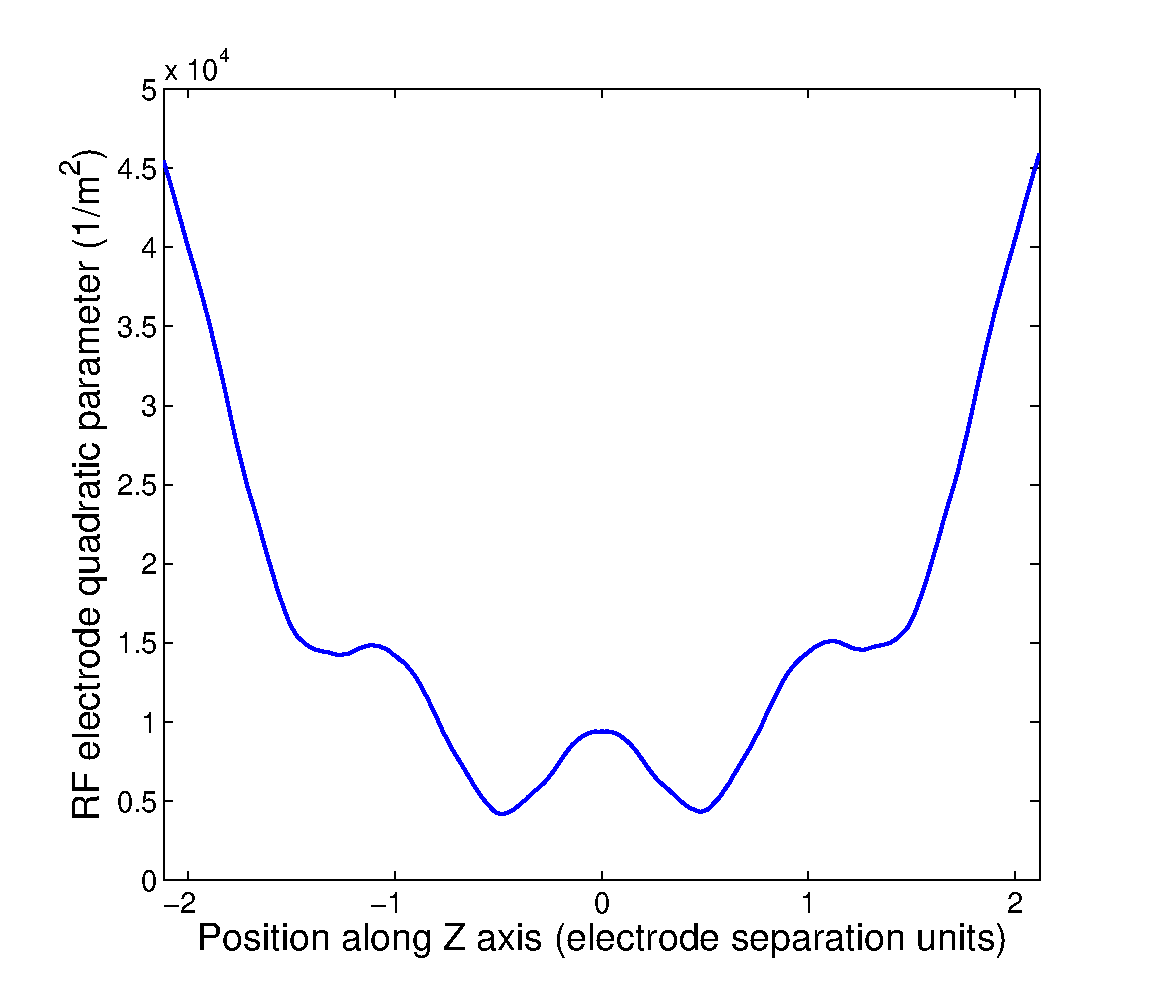
\includegraphics[width=7cm]{chapter2/liverpool/pseudopotz_v3} & 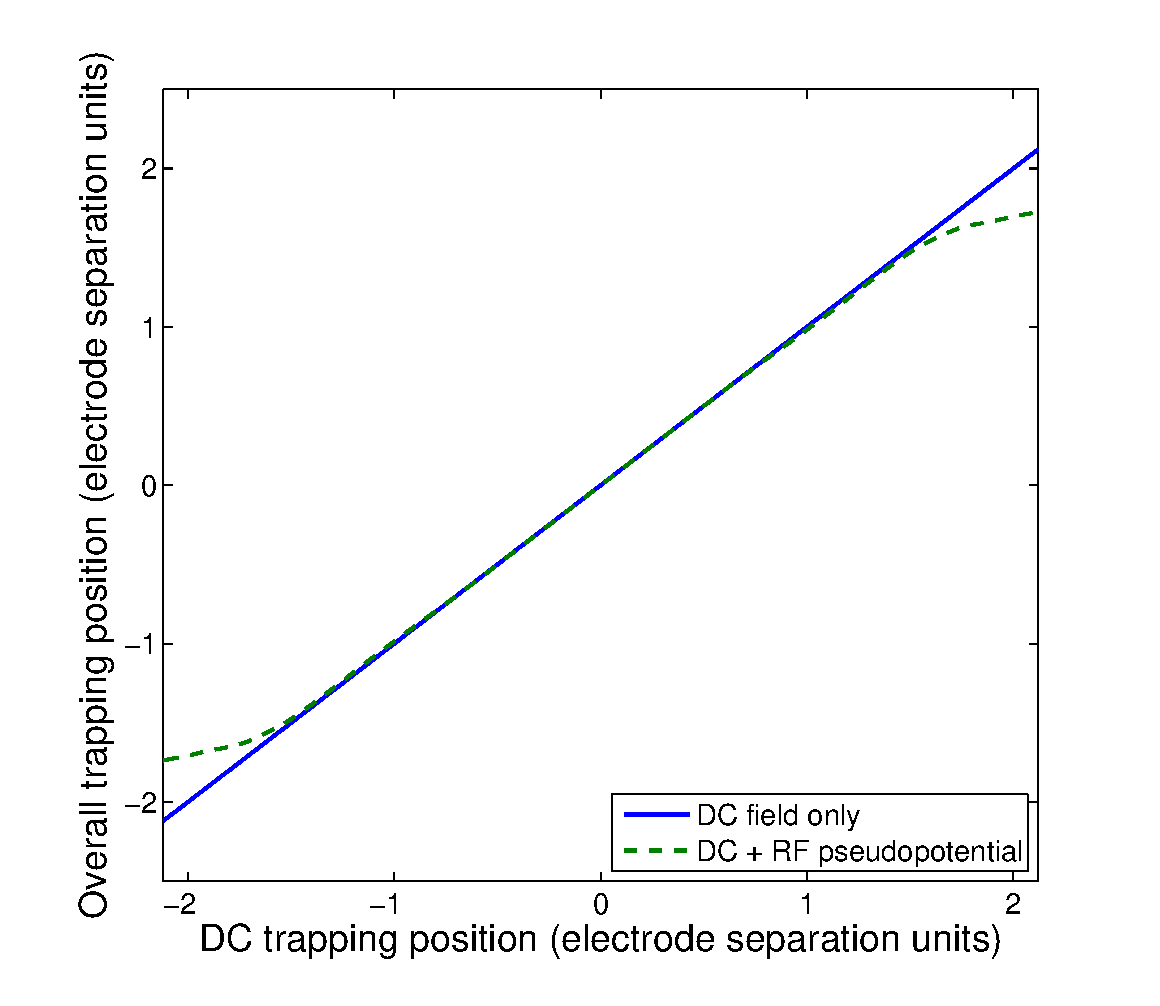
\includegraphics[width=7cm]{chapter2/liverpool/trapping_pos_v3} \\


%%%%%%%%%%%%%%%%%%
%\begin{figure}[h!t]
%\begin{center}
%$\begin{array}{cc}
%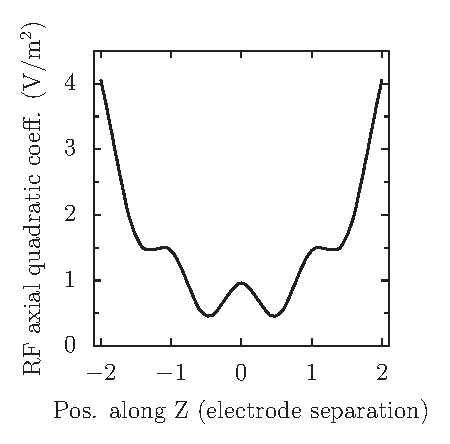
\includegraphics{chapter2/liverpool/liverpool_rf_quadcoeff} & 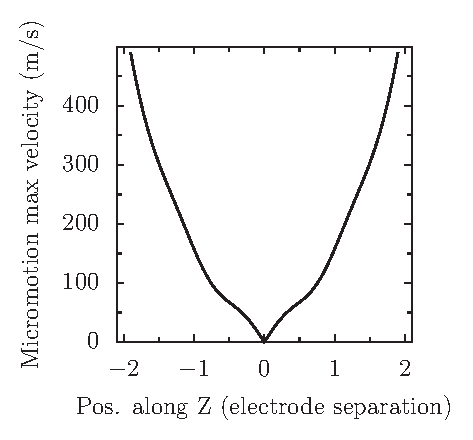
\includegraphics{chapter2/liverpool/liverpool_x_microvmax} \\
%\end{array}$
%\end{center}
%\caption[Effect of RF electrodes in the axial direction in the Liverpool trap]{(Left) the squared-gradient of the electric potential generated by unit voltage on the RF electrode, as a function of position along the trap axis $|\bigtriangledown \phi_{\rm rf}(z)|^2$, see equation~\ref{eq:pseudopot}. The shielding effect of the DC electrodes is visible as ``bumps'' in the function at the position of the DC electrodes. (Right) The estimated micromotion of the ion in the $Z$ direction due to the non-zero RF axial quadratic coefficient, when $\omega_{\rm dc}/2\pi = 300 \kHz$,  $V_{\rm rf} = 200V$ and $\Omega/2\pi = 5.92\MHz$, a typical set of operating parameters.
%%The position of the pseudo-potential well as a function of the position of the DC potential well along the trap axis, when $\omega_{dc}/2\pi = 300 \kHz$,  $V_{rf} = 200V$ and $\Omega/2\pi = 5.92\MHz$, a typical set of operating parameters. The RF displaces the ion significantly in the region of electrode distances $\pm 2$ (Electrodes \#2,\#6).
%}
%\label{fig:rfaxialeffect}
%\end{figure} 
%%%%%%%%%%%%%%%%




%%%%%%%%%%%%%%%%%
\begin{figure}[!t]
\begin{center}
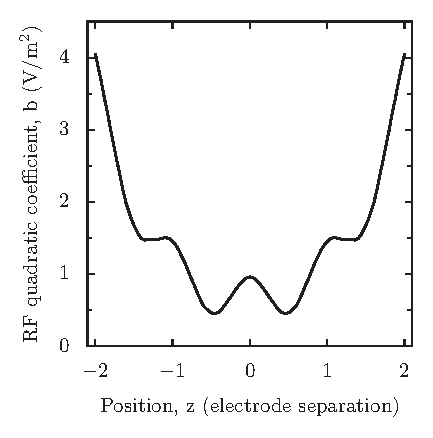
\includegraphics{chapter2/liverpool/liverpool_rf_quadcoeff_v2}
\end{center}
\caption[Axial component of fields generated by the RF electrodes]{
The quadratic coefficient $b$ in the expansion of the RF field along the Z axis, as a a function of position along Z (see Equation~\ref{eq:rfcoeffs}). The shielding effect of the DC electrodes appears as ``bumps'' at the position of the DC electrodes.
%The  position along the trap axis $|\nabla \phi_{\rm rf}(z)|^2$, see equation~\ref{eq:pseudopot}. The shielding effect of the DC electrodes appears as ``bumps'' in the function at the posit
%The squared-gradient of the electric potential generated by unit voltage on the RF electrode, as a function of position along the trap axis $|\nabla \phi_{\rm rf}(z)|^2$, see equation~\ref{eq:pseudopot}. The shielding effect of the DC electrodes appears as ``bumps'' in the function at the position of the DC electrodes.
}
\label{fig:rfaxialquad}
\end{figure} 
%%%%%%%%%%%%%%%%%
%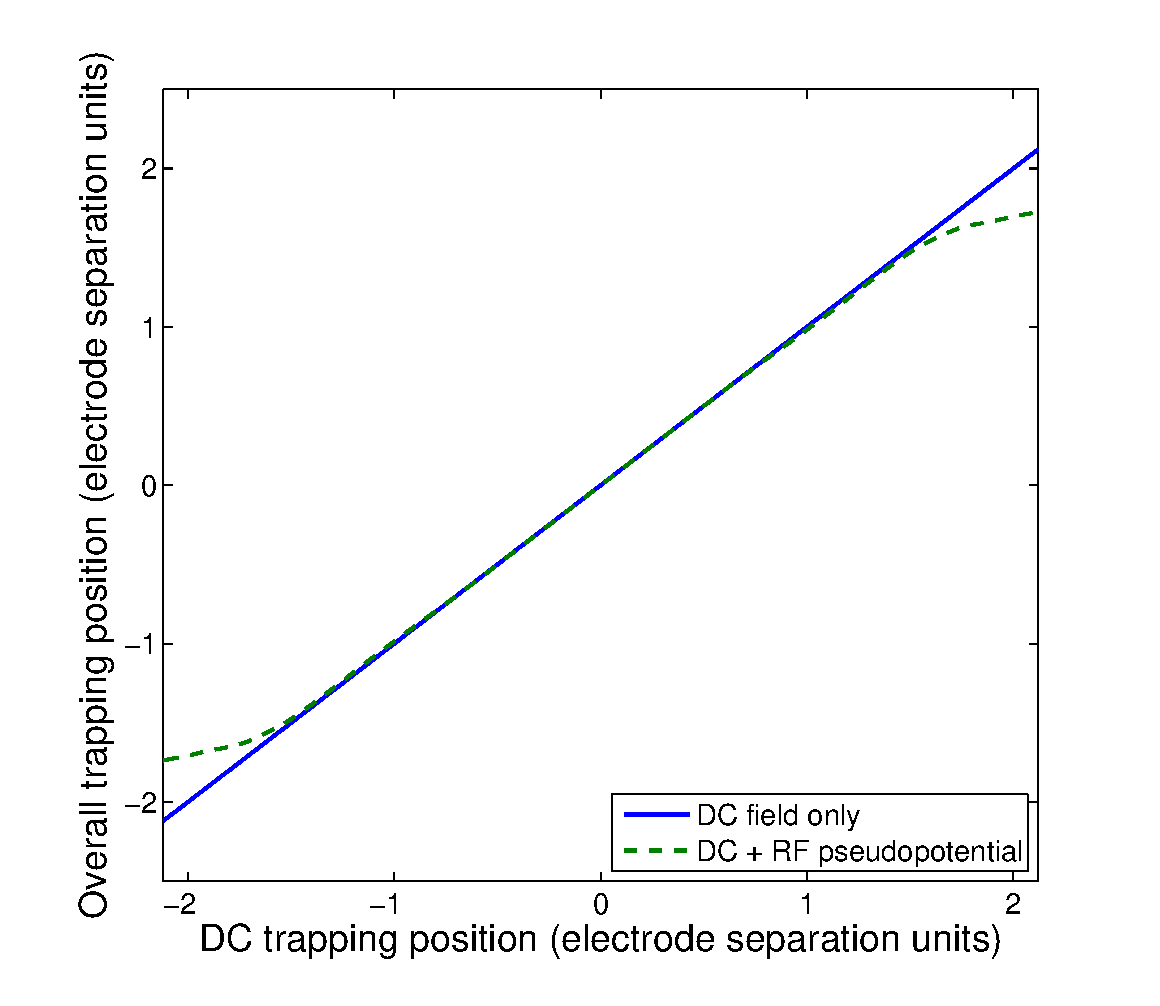
\includegraphics{chapter2/liverpool/trapping_pos_v3} & 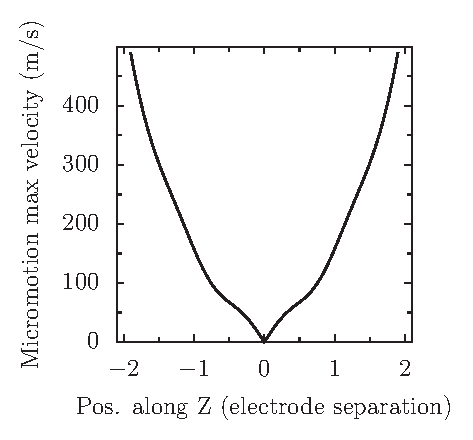
\includegraphics{chapter2/liverpool/liverpool_x_microvmax} \\
\begin{figure}[!t]
\begin{center}
$\begin{array}{cc}
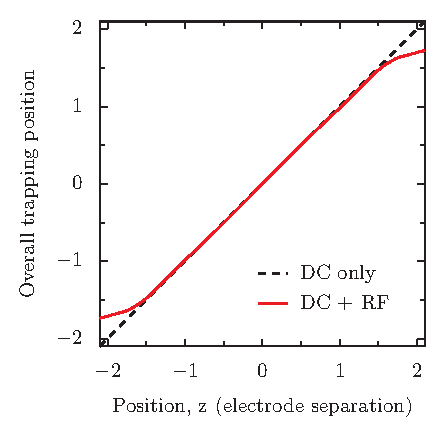
\includegraphics{chapter2/liverpool/liverpool_trapping_pos_v2} & 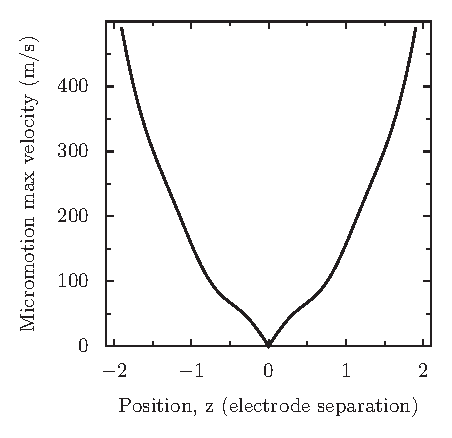
\includegraphics{chapter2/liverpool/liverpool_x_microvmax_v2} \\
\end{array}$
\end{center}
\caption[Effect of RF electrodes on axial pseudo-potential and micromotion]{(Left) The position of the pseudo-potential well as a function of the position of the DC potential well along the trap axis. (Right) The estimated micromotion of the ion in the Z direction due to the non-zero RF axial quadratic coefficient. In both cases, parameters are set to typical operating values: $\omega_{\rm dc}/2\pi = 300 \kHz$,  $V_{\rm rf} = 200V$ and $\Omega/2\pi = 5.92\MHz$. 
%The position of the pseudo-potential well as a function of the position of the DC potential well along the trap axis, when $\omega_{dc}/2\pi = 300 \kHz$,  $V_{rf} = 200V$ and $\Omega/2\pi = 5.92\MHz$, a typical set of operating parameters. The RF displaces the ion significantly in the region of electrodes $\pm 2$.
}
\label{fig:rfaxialeffect}
\end{figure} 
%%%%%%%%%%%%%%%


\subsection{Effect of manufacturing imprecision}
The actual trap geometry differs from the design. The most obvious difference is the displacement of one of the RF electrodes, possibly during assembly. Figure~\ref{fig:trapmodels} (right) shows the computer model of the trap with the twisted RF electrode. The displacement of the electrode was estimated from photographs, which suggests $\Delta z \approx 0.9\mm$,$\Delta x \approx 0.3\mm$ and a twist of $\theta \approx 4.7\degree$ in the X-Z plane. Rather than reassemble the trap, it was decided to operate it with this substantial asymmetry, in order to learn whether in practice this degree of manufacturing imprecision is a problem. 
% (the structure is quite fragile.)
An additional defect, the two lines of DC electrodes appear to have been shifted relative to each other, along the trap axis, by as much as half an electrode width ($\approx 290\um$). Precise measurements of this shift and evaluating its implications still to be investigated.

First we simulated the trap with the displaced RF electrode. When compared to the benchmark simulations, the most notable difference was in the position of the RF minima in the radial directions (X and Y). Figure~\ref{fig:twist_rfmin} shows the position of the RF minima as a function of location along the Z axis, in the original design and the one with the twisted electrode.

The original design is symmetrical in the X direction (across the trap), thus the location of the RF minimum is at the trap centre. In the twisted electrode model, the symmetry is broken and the minimum is displaced, though through a relatively small distance ($\sim 1\um$ maximum). In the Y direction (perpendicular to the plane of the DC electrodes) the RF minimum is already displaced from the geometrical centre of the RF electrodes (which is the origin of the scale presented in Figure~\ref{fig:twist_rfmin}(right)). This is due to the symmetry breaking of the compensation electrodes. In the twisted electrode model the RF potential minimium is displaced by up to $6\um$\, compared to the benchmark model. The 4 compensation electrodes were designed to allow compensation for just this sort of contingency. With them, it is possible to match the DC minimum to the RF minimum for up to 2 different positions in the trap. 

\begin{figure}[t]
%\centering
%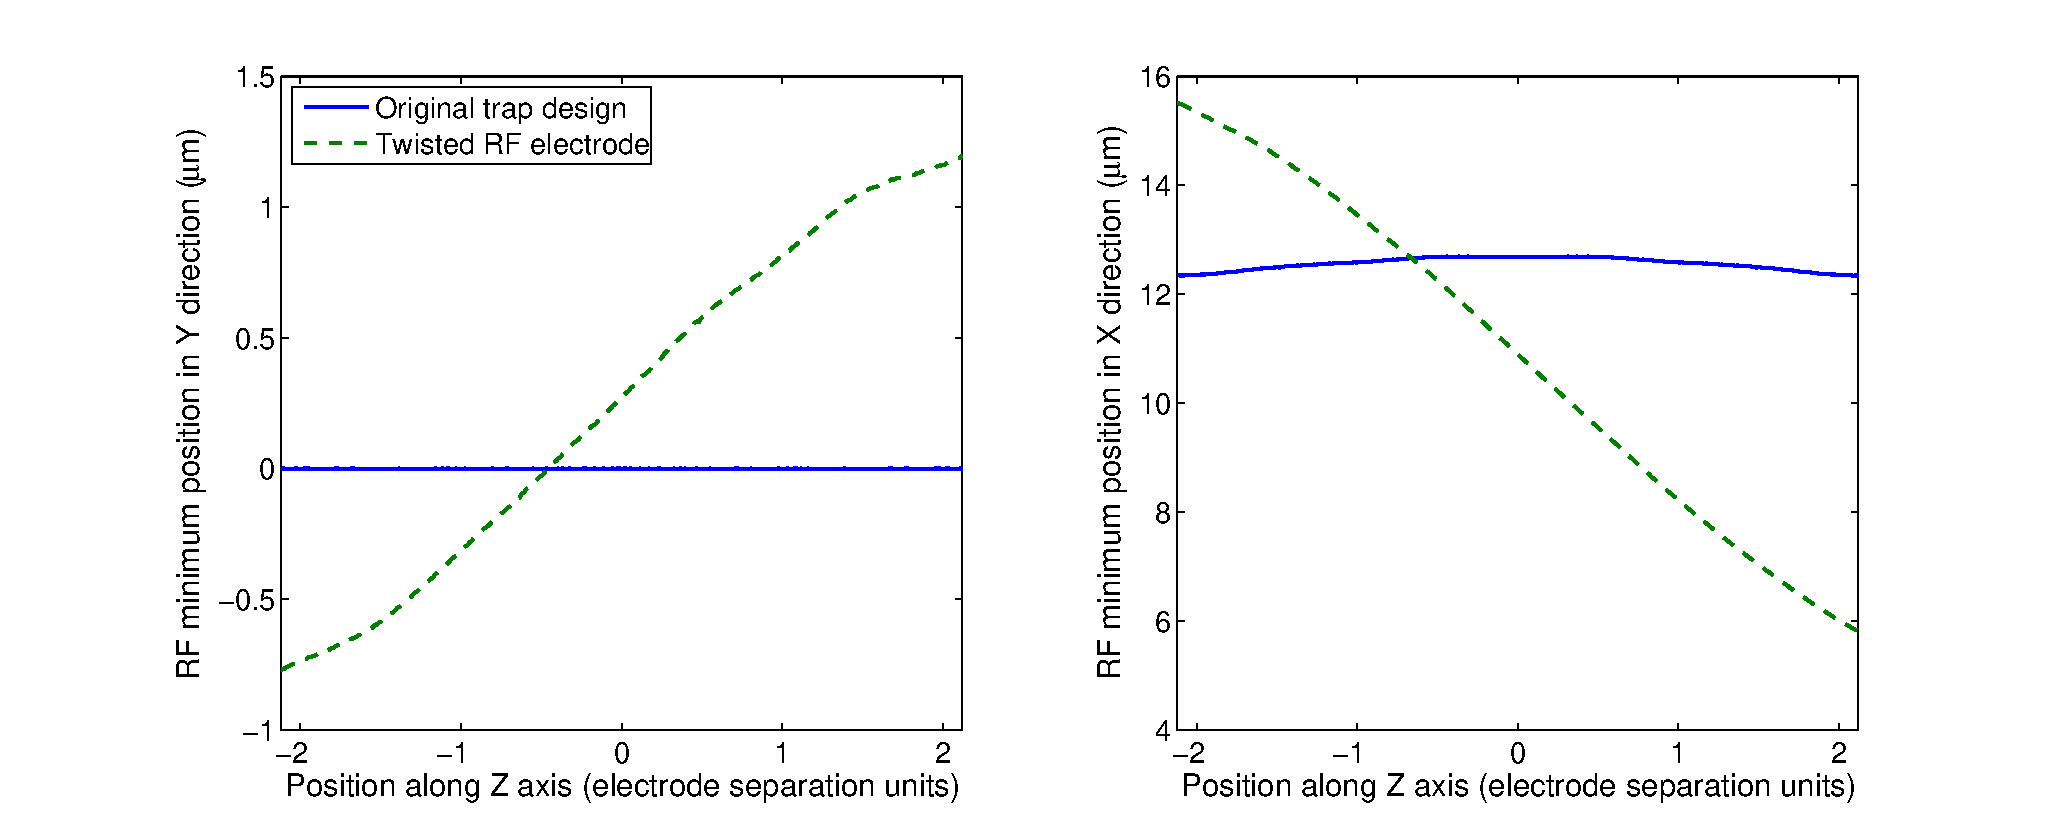
\includegraphics[width=15cm]{chapter2/liverpool/twist_rfmin_xy_v2}
\begin{center}
$\begin{array}{cc}
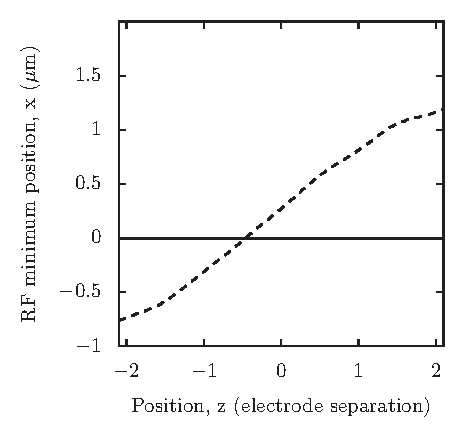
\includegraphics{chapter2/liverpool/rfminpos_x_v2} & 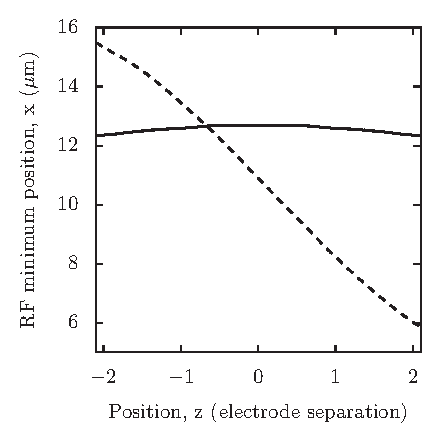
\includegraphics{chapter2/liverpool/rfminpos_y_v2} \\
\end{array}$
\end{center}
\caption[The position of radial RF minima in the Liverpool trap]{The position of the RF minimum as function of position along the trap axis, (left) in the X direction, across the trap, (right) in the Y direction, perpendicular to the plane of DC electrodes. The solid line is for the model as designed, the dashed line shows the effect of the twisted RF electrode. In the X direction the change is smaller ($\sim 1\um$ maximum), while in the Y direction the twist causes more substantial changes.}
\label{fig:twist_rfmin}
\end{figure} 

Recently the Liverpool trap has been tried in experimental conditions. Ions were trapped and initial trap frequency and compensation measurements were performed. 

%These initial results are consistent with the simulated trap parameters, however adjustments to the computational model are needed for better description of the trap geometry.

\section{The Sandia trap}
\label{sec:sandiaintro}

Another trap design was simulated, a DTO Module 4 ion trap (or ``Sandia trap'') provided by Sandia National Laboratories in Albuquerque, New Mexico, USA. It has a planar electrode arrangement on a chip carrier (Figure~\ref{fig:sandiatrap1}). 14 DC control electrodes are arranged around a $ 2000\um \times 400\um$ slot cut into the carrier. The DC electrodes have 7\um\, separation and have lengths of
% \{300\um, 200\um, 200\um, 100\um, 200\um, 200\um, 300\um\}.
100\um\, (centre electrode), 200\um\, (next two electrodes either side) and 300\um\, (the outermost electrodes).
Along the slot, there are 2 RF rails, approx. 10\um\, wide and 200\um\, apart. The sides of the slot were coated with gold and electrically connected to the common ground (``ground plane''). The trapping axis is along the slot, in between the RF rails. Experiments with this microfabricated segmented ion trap are presented in Chapters 5-7. More details of the trap hardware are given in Section~\ref{subsec:sandiatrap}.

As most of the simulation software tools were developed in detail with the Liverpool trap, applying the same analysis to a different trap design was relatively straightforward. The computational model of the trap was as in Figure~\ref{fig:sandia3d} and Figure~\ref{fig:sandiafield} shows a calculated electric field potential when the DC electrodes (as well as the ground plane) are grounded and the RF electrodes have a non-zero voltage applied to them.

By requiring the trapping frequencies to match the experimentally measured frequencies the voltage amplitude on the RF electrodes was calibrated in terms of RF input voltage, see Section~\ref{sec:ticleexperiment}. The trap was used for the ion shuttling experiments described in Section~\ref{sec:ionshuttle}, so we are interested in the geometrical factors $\gamma$ and $\mu$ for the Sandia trap. They are
\begin{align}
\gamma & \simeq 5 \times 10^{-5}, \\
\mu & \simeq 0.02.
\end{align}
Compared to the Liverpool trap, $\gamma$ is much smaller. This is because the DC electrodes are placed ``behind'' the RF electrodes from the ion's point of view; as a result the RF electrodes ``smooth'' out the potential created by the DC electrodes, reducing its quartic and higher order terms. Thus the Sandia trap is less suited for ion pair splitting than the Liverpool trap.
 


\begin{figure}[t]
\centering
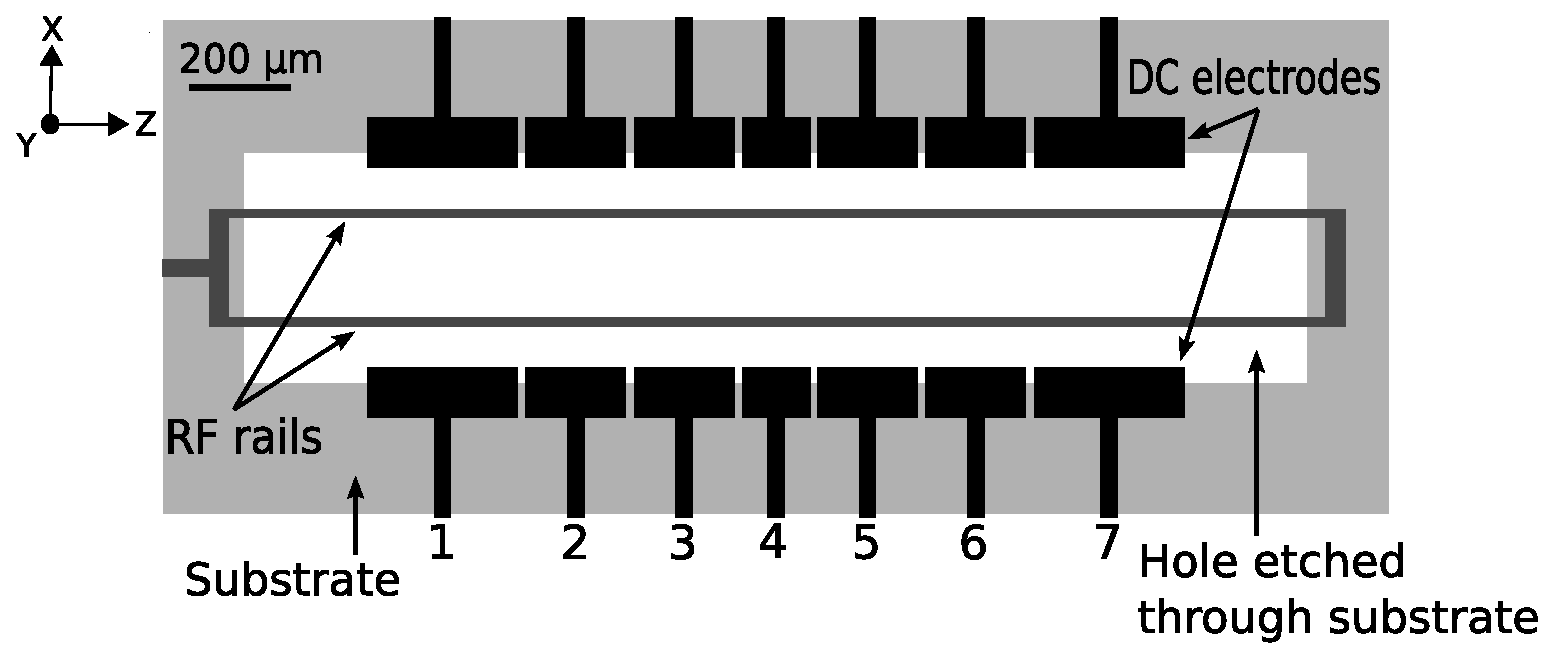
\includegraphics[width=11cm]{chapter4/sandia/trapscheme1d_v3}
\caption[Sandia trap schematics]{Schematics of the Sandia trap. Details are presented in Section~\ref{subsec:sandiatrap}.}
\label{fig:sandiatrap1}
\end{figure} 



As the results in Section~\ref{sec:ticleexperiment} show, the trap parameters predicted by the calculation are largely consistent with those determined by the experiment. There are discrepancies, though, e.g. in the prediction of the axial trap frequency (see Figure~\ref{fig:axialtickle}). These discrepancies are most probably due to simplifications and inaccuracies in our representation of the trap, as follows.

On the lower side of the trap, the etched substrate surface is covered with gold (the ``ground plane''), to eliminate charging of the dielectric material close to the trap. The position and angle of this surface, however, are not well determined due to the nature of the manufacturing process. Relatively minor issues include uncertainty in the size of the gaps between the adjacent electrodes, also the actual design of the RF rails is a complicated connecting ring structure, while in the simulation the RF rails were simplified to a pair of square rods with the appropriate dimensions.

To properly evaluate the effect of such misrepresentations of the geometry would require additional simulations. This becomes impractical because of the large number of parameters. In fact for most purposes the current model is adequate, as shown in Section~\ref{sec:ticleexperiment}. Experiments beyond the scope of this thesis, such as multiple ion shuttling, may require more detailed analysis.


%On the lower side of the trap, the etched substrate surface is covered with gold, to eliminate charging of the dielectric material close to the trap. The exact position and angle of this surface, however, is not well determined and has a large effect on the trap operation. The exact separation of the DC electrodes also has a $\approx 50\%$ uncertainty. The RF rails have a chain-like structure, being made of a large number of interconnected rings. Simulating this kind of structure is nevertheless beyond the capabilities of the software used, and probably would be subject to uncertainties as well. Currently the simulation treats the RF rails as two solid blocks and this model was sufficient for these initial calculations. Any more precise matching of predictions and experiments would require a large number of measurements and even more computing power. 
%


\section{Future traps}

Ion traps are being developed with even larger numbers of electrodes and to model these would strain the capabilities of our current simulations software. CPO is able to calculate up to 6000 elementary segments or divisions of electrodes. The simulation of the Sandia trap already uses up to 5960 segments, and comparing results of the calculation with models of the same trap with smaller number of elementary segments shows that this number cannot be decreased without loss in precision. Thus, for subsequent ion traps, more powerful Laplace equation solving software needs to be used. One such program is under development at the University of Ulm \cite{Huber2008}.

\begin{figure}[h!t]
\centering
%\includegraphics[width=14cm]{chapter2/sandia3d_v3}
\includegraphics[width=14cm]{chapter2/sandia3d_v4}
\caption[Computational model of the Sandia trap]{The 3D computational model of the Sandia trap, created in Matlab. The end section of the DC electrodes, the parallel portion of the RF rails and the ground plane on the side of the hole through the substrate is included (see Figure~\ref{fig:sandiatrap1}). }
\label{fig:sandia3d}
\end{figure} 

\begin{figure}[h!t]
\centering
%\includegraphics[width=14cm]{chapter2/sandiafield_v2}
%\includegraphics[width=14cm]{chapter2/sandiafield_v3}
\includegraphics[width=14cm]{chapter2/sandiafield_v4}
\caption[Calculation of the electric field in the Sandia trap]{Electric field due to a fixed voltage on the RF electrodes. Cross section in the X-Y plane, as shown in Figure~\ref{fig:sandiatrap1}.}
\label{fig:sandiafield}
\end{figure} 


%
%\begin{figure}[h!t]
%\centering
%
\includegraphics[width=10cm]{chapter2/LucentTrapSmall}
%\caption[Lucent trap]{}
%\label{fig:sandiatrap1}
%\end{figure} 
%



